\documentclass[t, 11pt]{beamer}
\pdfmapfile{+sansmathaccent.map}
%%% Работа с русским языком
\usepackage{cmap}				
\usepackage{mathtext} 				
\usepackage[T2A]{fontenc}		
\usepackage[utf8]{inputenc}			
\usepackage[english,russian]{babel}	

\usetheme{Ilmenau}
\usecolortheme{lily} % Цветовая схема



%%% Работа с картинками
\usepackage{graphicx}

\usepackage{csquotes}

\hypersetup{				
	colorlinks=true,       	
	linkcolor=blue,          
	citecolor=blue,       
	filecolor=magenta,      
	urlcolor=magenta           
}


\title{Классификация текстов}
\subtitle{topic modeling}
%\author{Чувакин Сергей}
\date{\today}
%\institute[<<Анализ больших данных в бизнесе, экономике и обществе>>]{<<Высшая школа экономики>>}
\institute{R meetup}
\begin{document}
	\frame[plain]{\titlepage}
	\section{Outline}
	
	\begin{frame}
		\frametitle{\insertsection} 
		\begin{block} {}
			 
			\hyperlink{l1}{\beamerbutton{Классификация текстов}}
		\end{block}
			\begin{block}{}
		\hyperlink{l2}{\beamerbutton{LSI}}
		\end{block}
				\begin{block}{}
		\hyperlink{l2}{\beamerbutton{Другие методы}}
		\end{block}
	\end{frame}
	

\subsection{Классификация текстов}
\begin{frame}
	\frametitle{\insertsection}
	\frametitle{\insertsubsection}  
	Text classification,  text tagging, text categorization, rubrication 
	\begin{itemize}
		\item Sentiment Analysis
		\item Topic Detection (modeling)
		\item Language Detection
		\item Exploratory Data Analysis
	\end{itemize}
\end{frame}


\begin{frame}
	\frametitle{\insertsection}
	\frametitle{\insertsubsection}  
	Techniques:
	\begin{itemize}
		\item distances
		\item KNN
		\item Kmeans
		\item PCA
		\item regression
		\item trees 
		\item etc (many other variations) 
	\end{itemize}
\end{frame}

\subsection{Topic modeling}
\begin{frame}
	\frametitle{\insertsection}
	\frametitle{\insertsubsection}  
	\textbf{Topic modeling} is a type of statistical modeling for discovering the abstract “topics” that occur in a collection of documents.
	 
	\vspace{0.5cm}
	
	Topic - in fact several important words.
	
	\vspace{0.5cm}
	
	\begin{itemize}
	\item \emph{LSI}, LDA
	\item PLSA, HDP
\end{itemize}
	
\end{frame}

\subsection{LSI}
\begin{frame}
	\frametitle{\insertsection}
	\frametitle{\insertsubsection}  
	\textbf{LSI} - topic modeling techniques based on SVD decomposition. 
	
	\vspace{0.5cm}
	
	\begin{itemize}
	\item Easy to understand
	\item Easy to specify
	\item Fast
\end{itemize}	
	\vspace{0.5cm}

\end{frame}


\begin{frame}
	\frametitle{\insertsection}
	\frametitle{\insertsubsection}  
	Pipeline:
	
	\vspace{0.5cm}
	input: corpus of documents, number of topics (n).
	\vspace{0.5cm}
	
	\begin{itemize}
		\item Normalization, preprocessing
		\item Matrix (M) doc-term via BOW 
		\item SVD decomposition 
		\item get 3 matrices $M=U\times\Sigma\times V^\intercal$  
	\end{itemize}	
	\vspace{0.5cm}
	
\end{frame}
\begin{frame}
	\frametitle{\insertsection}
	\frametitle{\insertsubsection}  
	Decomposition notation:

	\vspace{0.5cm}
	
	\begin{itemize}
		\item M - initial matrix document$\times$terms .
		\item U - docs$\times$topics.
		\item $\Sigma$ - topics$\times$topics.
		\item $V^\intercal$ - topics$\times$terms.   
	\end{itemize}	
	\vspace{0.5cm}
	
\end{frame}

	\begin{frame}
	\frametitle{\insertsection}
	\frametitle{\insertsubsection}
	
	
	%\vspace{1cm}
	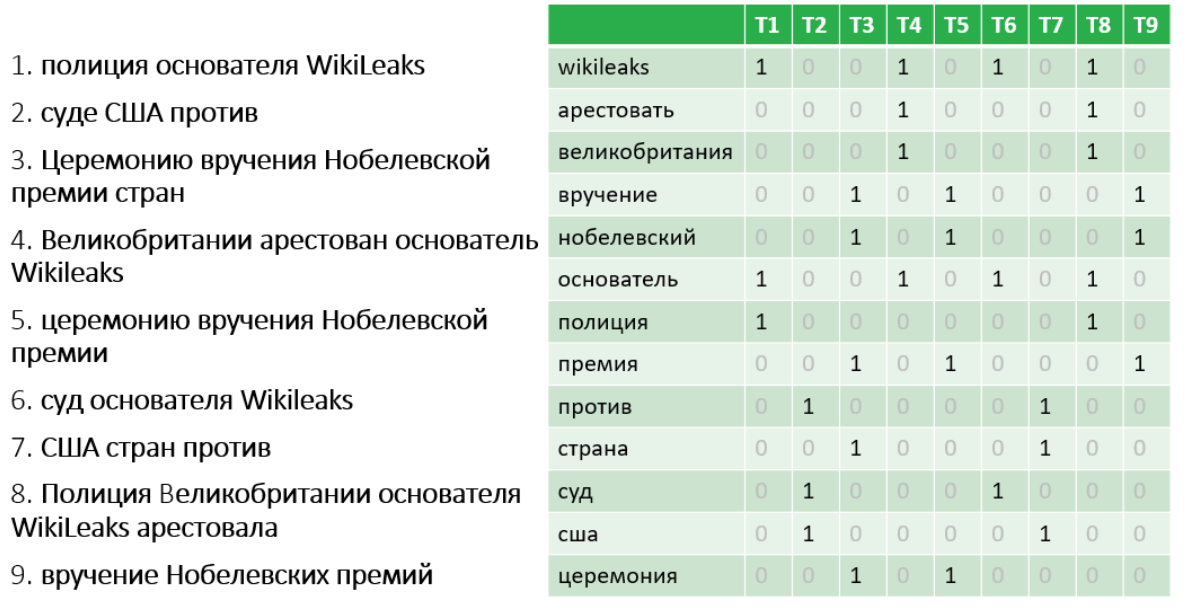
\includegraphics[width=0.9\linewidth]{init.png}
	%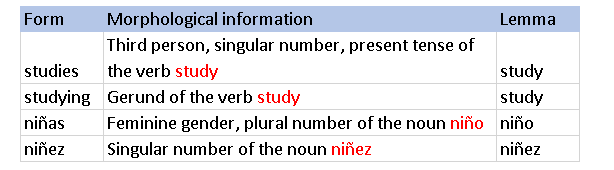
\includegraphics[width=0.7\linewidth]{lem.png}
\end{frame}


\begin{frame}
\frametitle{\insertsection}
\frametitle{\insertsubsection}


%\vspace{1cm}
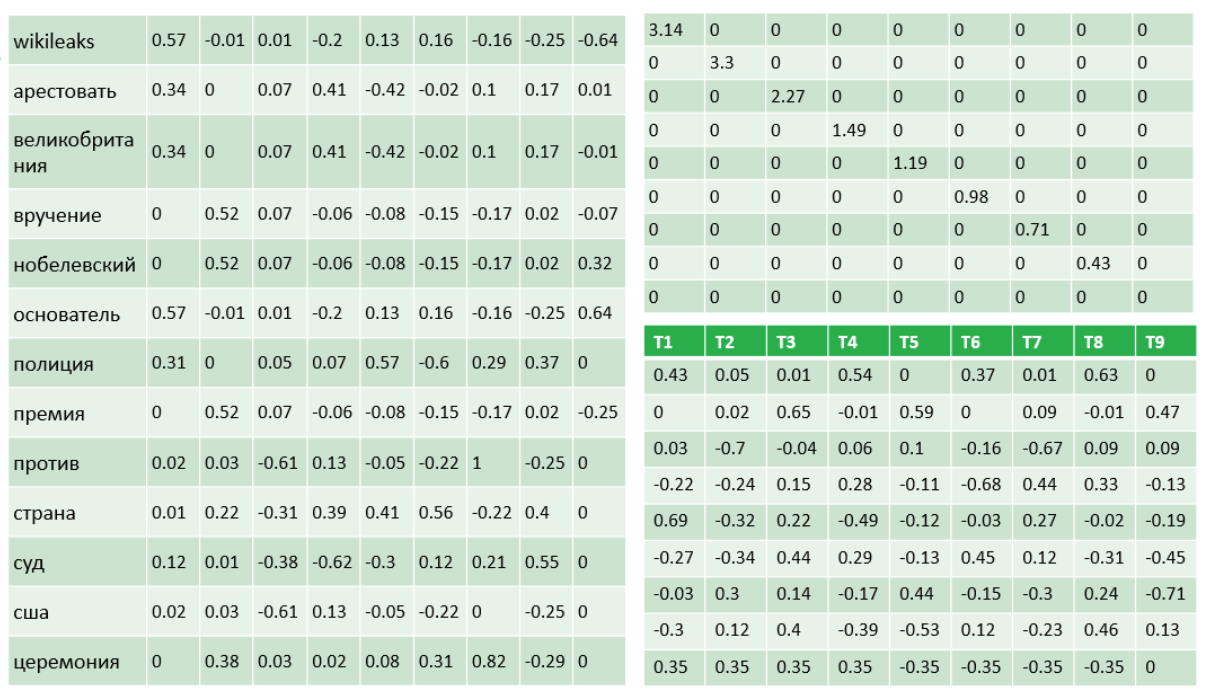
\includegraphics[width=0.9\linewidth]{decopm.png}
%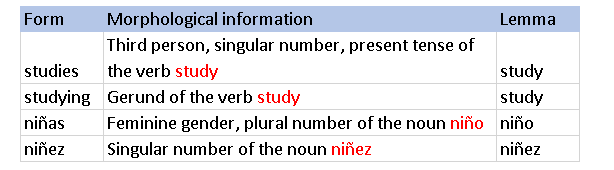
\includegraphics[width=0.7\linewidth]{lem.png}
\end{frame}

%
\begin{frame}
	\frametitle{\insertsection}
	\frametitle{\insertsubsection}
	
	
	%\vspace{1cm}
	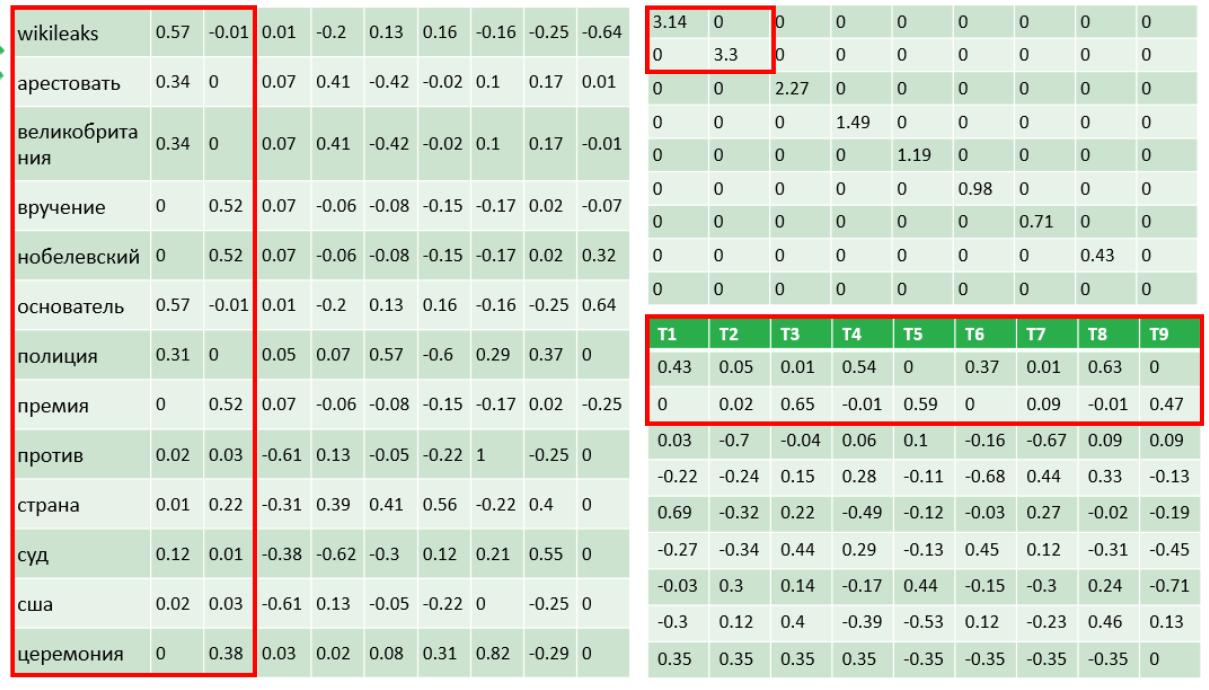
\includegraphics[width=0.9\linewidth]{deux.png}
	%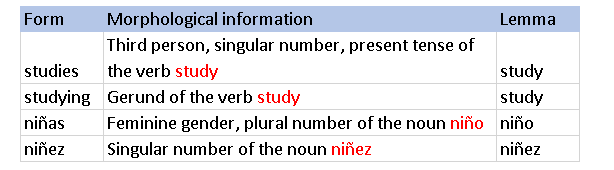
\includegraphics[width=0.7\linewidth]{lem.png}
\end{frame}

\subsection{Other methods}

\begin{frame}
	\frametitle{\insertsection}
	\frametitle{\insertsubsection}  
	LDA 
	
	\vspace{0.5cm}
	
	\begin{itemize}
		\item Slower
		\item More popular
		\item A prior knowledge about topic distribution
	\end{itemize}	
	\vspace{0.5cm}
	
\end{frame}

\begin{frame}
	\frametitle{\insertsection}
	\frametitle{\insertsubsection}  
	PLSA
	
	\vspace{0.5cm}
	
	\begin{itemize}
		\item Fast
		\item More "natural" coefficients
	\end{itemize}	
	\vspace{0.5cm}
	
\end{frame}


%	\begin{frame}
%	\frametitle{\insertsection}
%	\frametitle{\insertsubsection}  
%	Синонимы кватификаторов 
%	\begin{center}
%		\begin{table}[]
%			\begin{tabular}{c|c|c}
%				\hline
%				Синоним &Расшифровка &Квантификатор \\
%				\hline
%		+ & 1 и более раз &\{1,\}   \\
%		* & 0 и более раз &\{0,\}   \\
%
%		? &  0 или 1 раз& \{0,1\}  \\
%  
%			\end{tabular}
%		\end{table}
%	\end{center}
%\end{frame}

%\begin{frame}
%	\frametitle{\insertsection}
%	\frametitle{\insertsubsection}  
%	Чтобы убрать жаность необходимо добавить ?
%	
%	\vspace{0.5cm}
%	
%	Строка на вход  <<( dfghvb ) sdvsd ( sdcvkjnh ) sdvsd ( dkjhvgr ) sdvfv.>>
%	
%	\vspace{0.5cm}
%	
%	шаблон: r"$\backslash$(.+?$\backslash$)"
%	
%	\vspace{0.5cm}
%	
%	на выходе: ['dfghvb', 'sdcvkjnh', 'dkjhvgr']
%	
%\end{frame}



%	\begin{frame}
%	\frametitle{\insertsection}
%	\frametitle{\insertsubsection}
%	
%	
%	\vspace{1cm}
%	\includegraphics[width=0.9\linewidth]{page2.png}
%	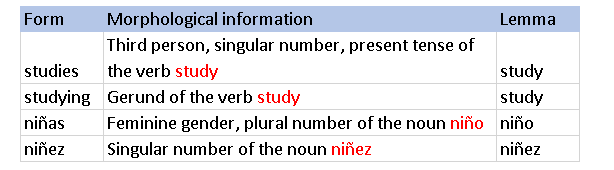
\includegraphics[width=0.7\linewidth]{lem.png}
%\end{frame}
\end{document}